\chapter{The ND-LAr Cryostat}
\label{ch:cryostat}


%%%%%%%%%%%%%%%%%%%%%%%%%%%%%%%%
\section{Overview of the Cryostat}
\label{sec:cryost-ovvw}
The DUNE Near Detector (ND) liquid argon cryostat is responsible for maintaining the cryogenic environment required for the liquid argon TPC modules.  Similar to other large cryostats for LArTPCs, the DUNE ND LAr cryostat utilizes a stainless steel membrane containment system with an external superstructure to support the hydrostatic and pressure loads of liquid argon.
The DUNE ND LAr cryostat is unique compared to most membrane cryostats for liquid argon.  Firstly, it is mounted to the PRISM movement system, which will translate the cryostat along the length of the Near Site cavern hall to sample the delivered neutrino beam at various locations.  Secondly, the downstream cryostat wall utilizes a low-density window construction to minimize attenuation of muons that exit the active region of the LArTPC array.  The design of this low density window is covered in Section 2.2.1 and its implications of membrane cryostat safety are covered in Section 2.2.2.



%%%%%%%%%%%%%%%
\subsection{Introduction and Scope}
\label{sec:cryost-ovvw-intro}
This section covers the liquid argon cryostat that will house the LArTPC array at the DUNE Near Site.  The cryostat maintains a liquid argon bath for operation of the TPCs.  The following sections covers the design and requirements of the cold and warm containment structures, lid sections, interfaces, risks, schedule and installation activities.


%%%%%%%%%%%%%%% Not in Tim's new organization
\subsection{Principle of Operation}
\label{sec:cryost-ovvw-op}

%\begin{dunetable}
%[Placeholder for parameter table]
%{cc}
%{tab:table-cryost-params}
%{Placeholder for Parameter Table - it will be generated from a spreadsheet}
%Rows & Counts \\ \toprowrule
%Row 1 & First \\ \colhline
%Row 2 & Second \\ \colhline
%Row 3 & Third \\ % no \colhline on final row
%\end{dunetable}

%%%%%%%%%%%%%%%
\begin{dunetable}
[Cryostat Parameters]
{lll}
{tab:table-cryost-params}
{LAr Cryostat Design Parameters}
Design Parameter            & Value & Notes \\ \toprowrule
Inner Volume                & $5500\times 6000 \times 9000 \mbox{mm}^2$ &height $\times$ width $\times$ length \\ \colhline
Tank Capacity               & 340 metric tonnes & Defined by cold membrane vessel \\ \colhline
Residual Heat Input         & $<10$ $\mbox{W}/\mbox{m}^2$       & \\ \colhline
Insulation Density          & 90  $\mbox{kg}/\mbox{m}^3$& \\ \colhline
Insulation Thickness        & 800 $\mbox{mm}$           & \\ \colhline
Maximum Allowable Pressure  & 350 $\mbox{mbarg}$        & \\ \colhline
Cavern Ambient Pressure     & 1020.355 $\mbox{mbara}$   & \\ \colhline
\end{dunetable}

\begin{dunefigure}[Cryostat Overall Dimensions]{fig:cryo_dim}
{Cryostat Overall Dimensions (mm).}
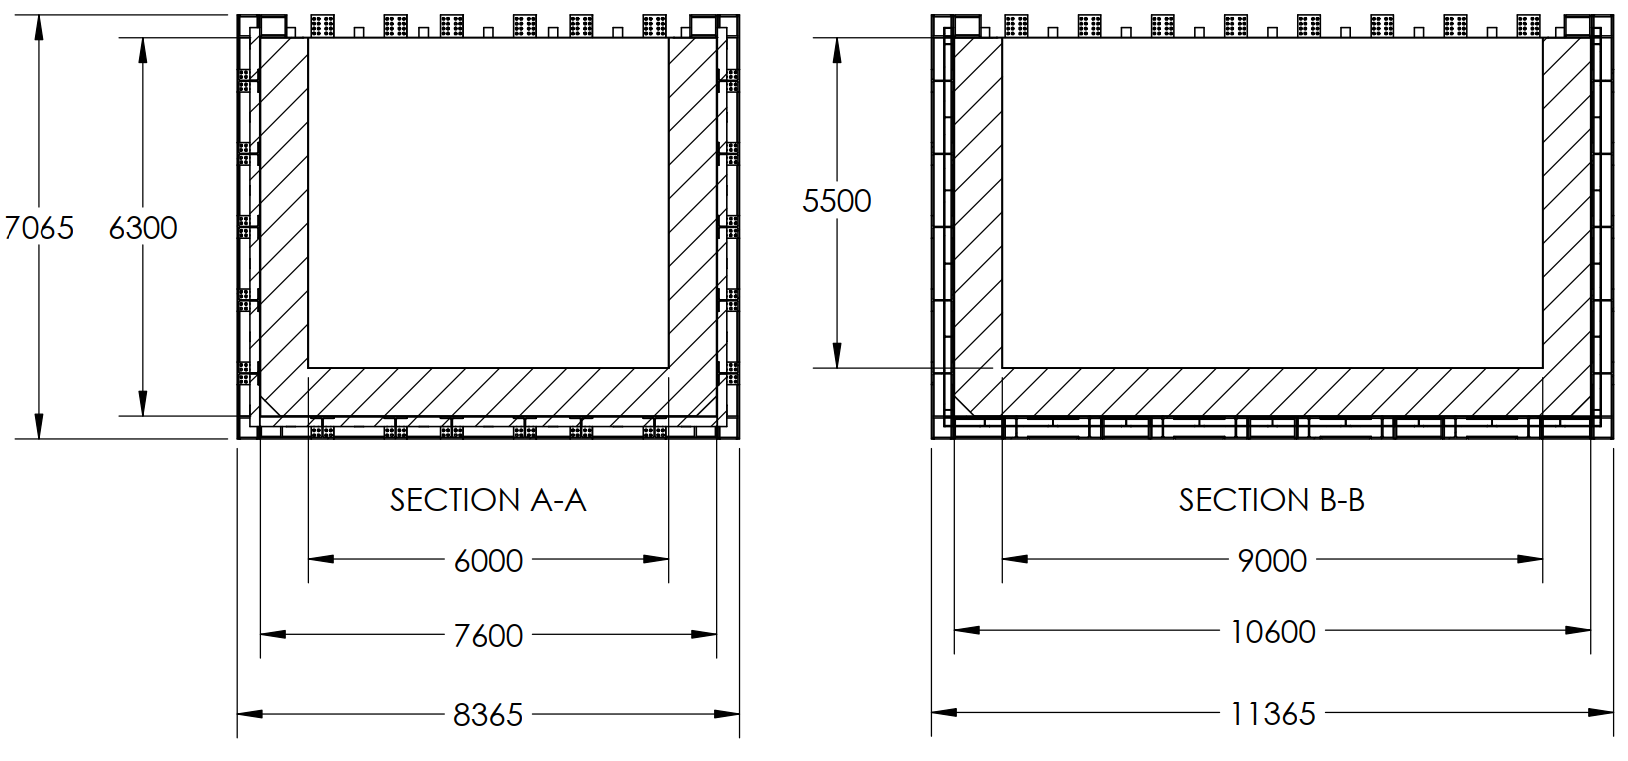
\includegraphics[width=0.9\textwidth]{cryostat_dimensions.png}
\end{dunefigure}

\begin{dunetable}
[Cryostat Parameters]
{llll}
{tab:table-cryost-dimensions}
{LAr Cryostat Structure Nominal Dimensions}
Parameter                            & Length (mm) & Width (mm)    & Height (mm) \\ \toprowrule
Membrane Flat Internal Dimensions & 9000    & 6000  & 5500 \\ \colhline
Warm Structure 10 mm Steel Skin Internal Dimensions  & 10600 & 7600  & 6300 \\ \colhline
External Steel Structure Dimesions          &     11365   & 8365  & 7065 \\
\end{dunetable}


\subsection{Design Parameters}
\label{sec:cryost-ovvw-param}
The cryostat is designed to meet the physics requirements of the \dword{dune} experiment. 
The important design parameters are given in Table~\ref{tab:table-cryost-params}. 

The cryostat overall dimensions are based on the required volume of liquid argon for the TPC detector, and the resulting structure required to support it.  The nominal external and internal dimensions for the cryostat are shown in Figure \ref{fig:cryo_dim}.

Nominal structure dimensions are also tabulated in Table 2.2 below.

\begin{itemize}
\item Size requirements
\item Containment requirements
\item Capabilities
\item Operating parameters
\end{itemize}




%%%%%%%%%%%%%%%Not in Tim's new organization
\subsection{Performance}
\label{sec:cryost-ovvw-perf}



%%%%%%%%%%%%%%%%%%%%%%%%%%%%%%%%
\section{System Design}
\label{sec:cryost-des}

%%%%%%%%%%%%%%%
\subsection{Composite Wall}
\label{sec:cryost-des-wall}
\fixme{highlight as unique feature}


%\begin{itemize}
%\item Requirement motivating composite window
%\item Composite window construction method
%\item Progressive prototyping program
%\item Composite window Procurement \& QAQC
%\end{itemize}

\subsubsection{Motivation for Composite Window}
The overarching requirement of the DUNE near detector (ND) is to identify $\nu_\mu$- and $\nu_e$-induced charged-current (CC) interactions and to measure the energy of the incident neutrino, over a range of neutrino energies relevant for oscillations, roughly 0.5-5 GeV. The precision of the energy measurement must equal or exceed that of the far detector (FD) so that measurements made at the ND can be extrapolated to the FD. Neutrino energy can be subdivided into two components, the lepton energy and the energy of the hadronic system, both of which must be precisely measured.  In the liquid argon near detector (ND-LAr), the active LAr volume is designed to be sufficiently large to fully contain the energy of the hadronic system, and to contain the outgoing electron in $\nu_e$ CC events. However, to cover the full energy range relevant for oscillations, the outgoing muon may have energy up to 5 GeV, which would travel $\sim 20$ m in LAr. For this reason, ND-LAr is functionally coupled to a muon spectrometer. The hadronic energy is measured by ND-LAr, and the muon energy is measured energy in ND-LAr and the downstream spectrometer. Muons which exit the active region of ND-LAr and stop in the inactive material between the two detectors cannot be measured to the required precision and must be excluded from analysis. This coupling makes the measurement especially sensitive to inactive material located in between the active volume of ND-LAr and the active volume of the spectrometer. To meet the physics requirements of the DUNE ND program, the total areal density of this inactive material must be less than 50 g/cm2 over at least 90\% of the coverage area, with uniformity better than 12\%.

\begin{dunefigure}[Muon reconstruction efficiency for $\nu_\mu$ CC in ND-LAr]{fig:eff_numucc}
{The efficiency for $\nu_\mu$ charged-current events in the ND-LAr fiducial volume to have a well-reconstructed muon and hadronic system, shown as a function of muon kinetic energy for forward muons with $\theta_\mu< 20^\circ$. Events are excluded when the muon stops in the passive material between ND-LAr and the spectrometer, which is 50 $\mbox{g}/\mbox{cm}^2$ (left), 100 $\mbox{g}/\mbox{cm}^2$ (center), and 150 $\mbox{g}/\mbox{cm}^2$ (right). At high energy, the acceptance deviates from unity due to muons at higher angles missing the downstream spectrometer.}
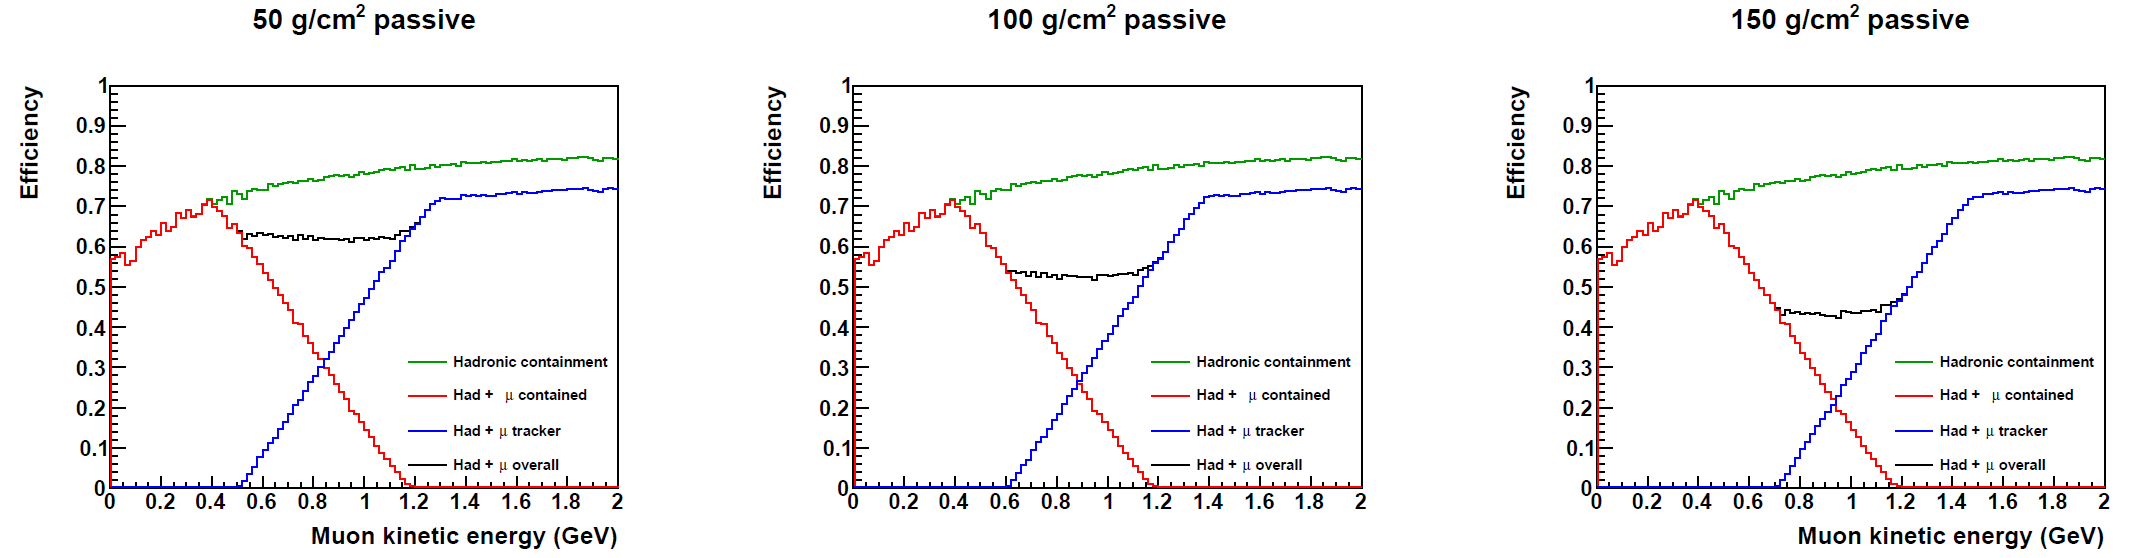
\includegraphics[width=0.95\textwidth]{numu_cc_efficiency.png}
\end{dunefigure}

\subsubsubsection{Event reconstruction Requirements}
The required muon momentum resolution of the near detector is set by the momentum resolution achievable in the far detector. Oscillation parameters are inferred by comparing observed neutrino energy spectra in the FD to predictions. These predictions are constrained by ND data. If the energy resolution of the ND is worse than that of the FD, then theoretical models must be used to correct the predictions. Because of the nontrivial shape of the FD energy spectra (which is caused primarily by oscillations themselves), these corrections are sensitive not only to the detector model but also to neutrino interaction modeling. In order to extrapolate ND data to the FD without introducing additional modeling uncertainties, it is required that the ND energy resolution be equal or superior to that of the FD.

In the far detector (FD), muon momentum is reconstructed either by range or by multiple coulomb scattering (MCS). For muon momentum between 0.5 and 5 GeV, the resolution is 4\% by range and 15\% by curvature. Due to the large size of FD modules, the majority of muons will be reconstructed by range; a 2.5 GeV muon travels approximately 10 m in liquid argon and will be contained in a single FD module $\sim 80\%$ of the time. The resolution for reconstruction by range is used as the requirement for the ND. This 4\% is relatively at as a function of true momentum in the oscillation region. 

Muons that stop in the ND-LAr active region will be reconstructed by range in liquid argon. Muons will also be reconstructed primarily by range when they exit the ND-LAr detector and enter the temporary muon spectrometer (TMS), or the calorimeter of the ND-GAr detector. The ND-LAr active volume is 5 m long in the direction nearly parallel to the neutrino beam. To reject front-entering events, the most upstream 50 cm is excluded from analysis. To contain hadronic showers, the downstream 150 cm is also excluded. Some neutrino interactions produce minimal hadronic activity and can be analyzed when they occur within those 150 cm, but this is not possible in general, and attempting to analyze all interactions in this volume would introduce large uncertainties due to interaction modeling. Therefore we select CC $\nu_\mu$ events in a 300 cm region between 50 cm and 350 cm from the upstream face of the active volume. This means that for muons in the forward direction, the maximum path length in LAr is 450 cm, corresponding to a maximum muon kinetic energy of about 1.1 GeV. Above that energy, forward muons are never contained and must always be matched to tracks in the downstream spectrometer.

For 1 GeV muons, the 4\% resolution requirement means that the kinetic energy from range must be known to ~ 40 MeV, which corresponds to an upper bound of ~ 20 g/cm2 on the material traversed. If the uncertainty on the stopping point of the muon is greater than that, the momentum resolution will be dominated by that uncertainty rather than by fluctuations in ionization. For the inactive material in between the detectors, this 20 g/cm2 is not possible, so we instead exclude from analysis muons which exit the active LAr but do not enter the spectrometer. This exclusion causes a dip in the ND acceptance as a function of muon energy, which is shown in Figure \ref{fig:eff_numucc}. The dip is broadened by the fact that we can analyze interaction vertices over a 300cm region in ND-LAr, so muons that stop in the passive material have between 400 and 1100 MeV kinetic energy depending on the location of the vertex. The total thickness of passive material determines the minimum energy where tracker-matched muons begin to turn on. The fraction of muons which fall into the dip is related to the ratio of the total passive material thickness to the total thickness of the fiducial volume, which is 420 g/cm2.

\begin{dunefigure}[Muon reconstruction efficiency vs. q0,q3,Enu=2.0-2.5 GeV]{fig:eff_numucc_q0q3_2025GeV}
{Left: the efficiency for $\nu_\mu$ charged-current events in the ND-LAr fiducial volume to have a well-reconstructed muon and hadronic system, shown as a function of three-momentum and energy transfer to the nuclear system for $2.0 < E_\nu < 2.5\;\mbox{GeV}$ for 100 $\mbox{g}/\mbox{cm}^2$ passive material. Right: The ratio of the efficiency with 150 $\mbox{g}/\mbox{cm}^2$ passive material to 100 $\mbox{g}/\mbox{cm}^2$.}
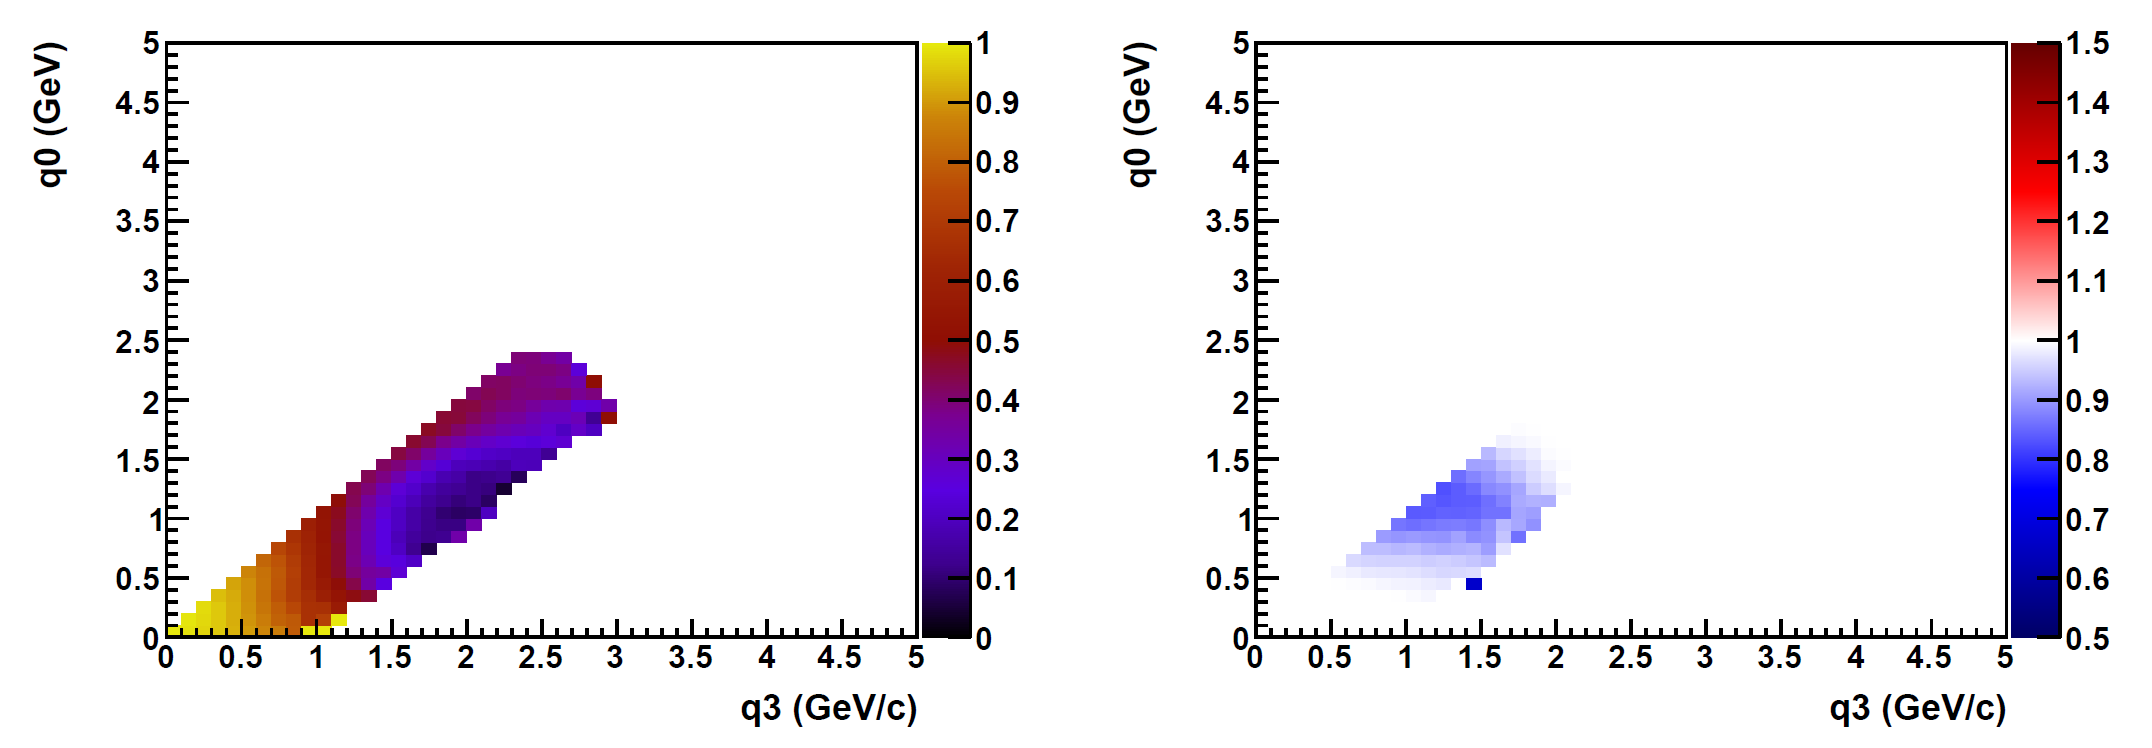
\includegraphics[width=0.95\textwidth]{graphics/numu_cc_efficiency_q0q3_2.0-2.5GeV.png}
\end{dunefigure}

\begin{dunefigure}[Muon reconstruction efficiency vs. q0,q3, Enu=3.5-4.0 GeV]{fig:eff_numucc_q0q3_3540GeV}
{Left: the efficiency for $\nu_\mu$ charged-current events in the ND-LAr fiducial volume to have a well-reconstructed muon and hadronic system, shown as a function of three-momentum and energy transfer to the nuclear system for $3.5 < E_\nu < 4.0\;\mbox{GeV}$ for 100 $\mbox{g}/\mbox{cm}^2$ passive material. Right: The ratio of the efficiency with 150 $\mbox{g}/\mbox{cm}^2$ passive material to 100 $\mbox{g}/\mbox{cm}^2$.}
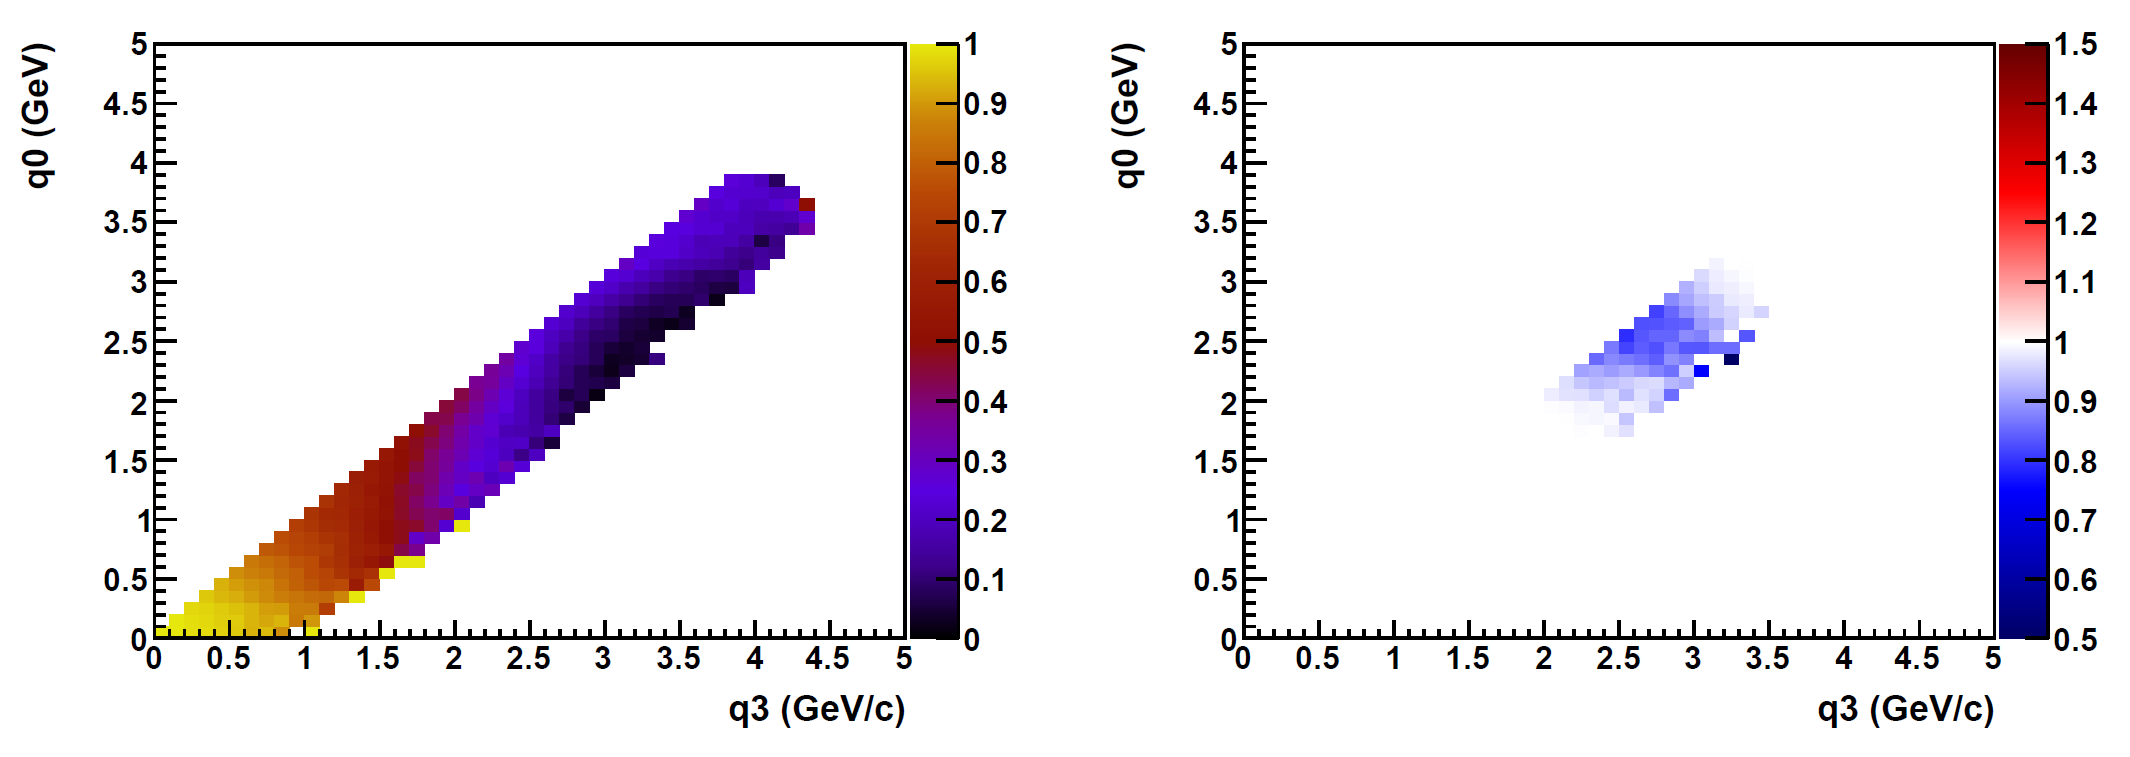
\includegraphics[width=0.95\textwidth]{graphics/numu_cc_efficiency_q0q3_3.5-4.0GeV.png}
\end{dunefigure}

\begin{dunefigure}[Fraction of total cross section with less than 10\% efficiency]{fig:eff_numucc_10pct}
{The fraction of the total cross section in a region of $q_0-q_3$ space with efficiency below 10\%, as a function of neutrino energy. This is essentially the size of the black regions in Figures \ref{fig:eff_numucc_q0q3_2025GeV} and \ref{fig:eff_numucc_q0q3_3540GeV}, weighted by the total cross section.}
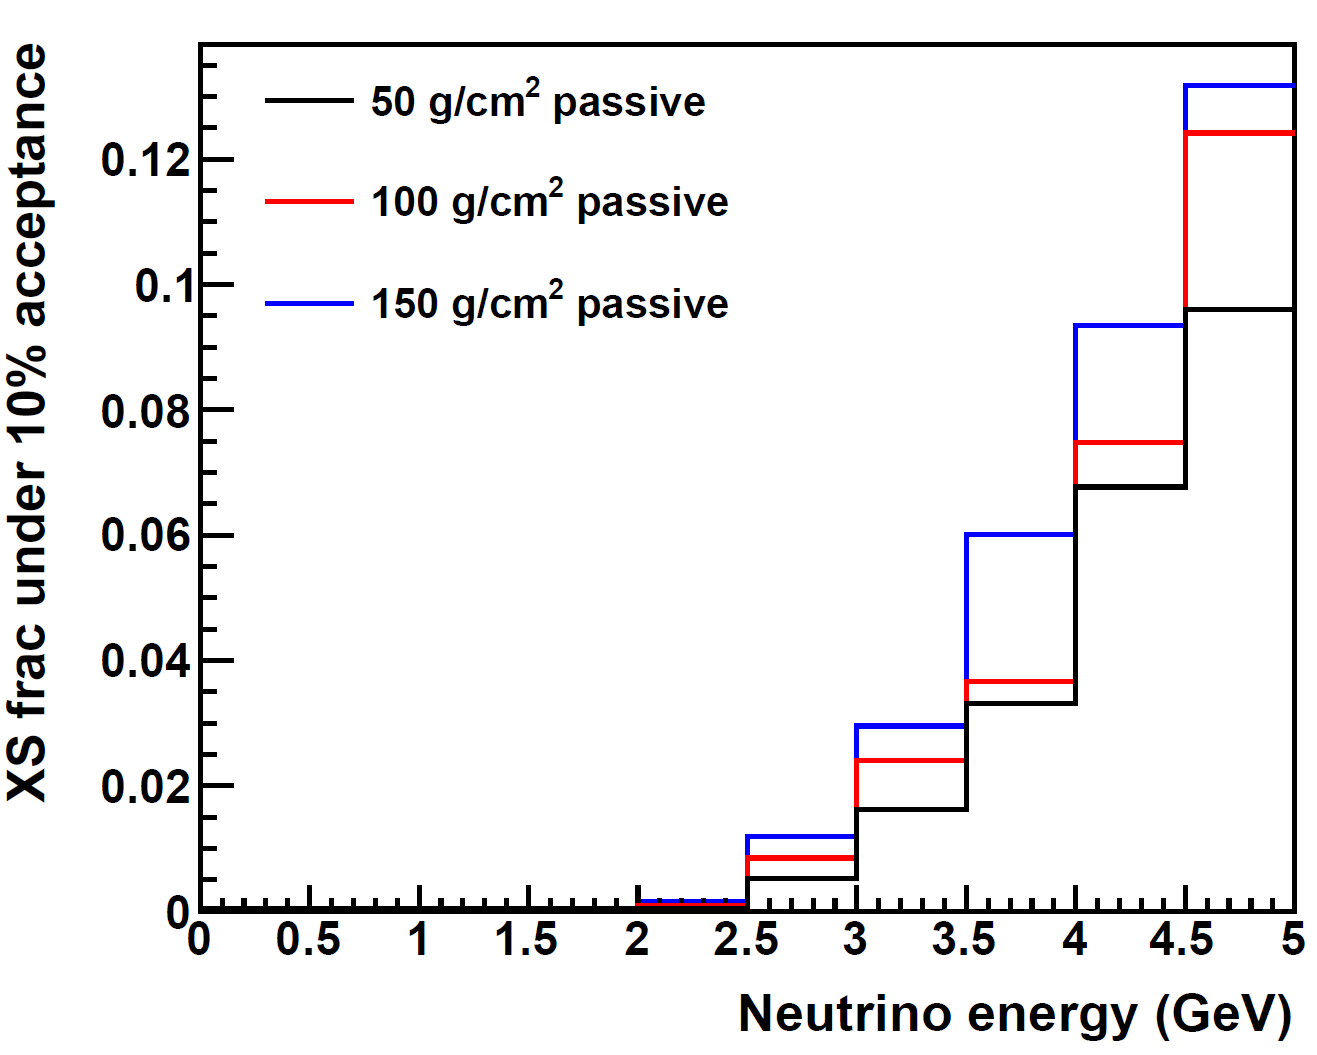
\includegraphics[width=0.65\textwidth]{graphics/numu_cc_efficiency_10pct.png}
\end{dunefigure}


\subsubsubsection{Cryostat Wall Thickness}
Muon acceptance is defined as either stopping in the ND-LAr active volume, or penetrating into the active volume of the downstream spectrometer (TMS or ECAL). Starting at muon kinetic energy of 0.4, forward muons in the most downstream region of the fiducial volume begin to exit the active LAr. For muons of a given kinetic energy between 0.4 and about 1.2 GeV, there is essentially a dead region in the LAr fiducial volume, where tracks originating in this region will terminate in the passive material and their momenta cannot be measured at the required precision. The width of this dead region is proportional to (and exactly equal to, for muons that are exactly 6° above the neutrino beam) the total areal density of the passive material between the two detectors. As muon energy loss is proportional to the areal density traversed (measured in g/cm2), it is the integrated density along a straight-line trajectory connecting the two active volumes that impacts the physics. The electromagnetic radiation length and nuclear interaction length of the material in this region is irrelevant, because our physics analyses will not require tracking electrons or hadrons through this region.

The impact of the passive material on both muon and hadron reconstruction can be seen by looking at the efficiency to reconstruct both the muon and hadronic system as a function of energy transfer from the neutrino to the hadronic system, $q_0$, and three-momentum transfer, $q_3$. Neutrino interaction modeling issues map well onto this kinematic space; for full coverage of the neutrino cross section, it is critical that there not be any regions in this space where the ND efficiency is very low. For a given neutrino energy, $E_\nu$, the muon energy is related to the total hadronic energy $E_{had} = q_0$ by $E_\mu = E_\nu - q_0$. The muon angle is exactly forward when $q_0 = q_3$. Figure \ref{fig:eff_numucc_q0q3_2025GeV} shows the efficiency in this space for $2.0 < E_\nu < 2.5$ GeV and 100 g/cm2 total passive material, along with the relative change in the efficiency in increasing the passive material from 100 to 150 g/cm2. It is observed that losses are most significant in the forward region, as expected. Figure \ref{fig:eff_numucc_q0q3_3540GeV} shows the same thing for higher neutrino energy, $3.5 < E_\nu < 4.0$ GeV on the falling edge of the flux peak.


Regions of phase space with efficiency below 10\% are especially problematic. This typically means events can be reconstructed only in a very particular location within the detector, or only when the hadronic shower happens to be composed of certain final-state particles. In the DUNE-PRISM analysis, the method of using ND data itself to translate and rotate vertices in order to determine the efficiency correction with minimal dependence on interaction modeling breaks down when regions of phase space have such low acceptance. As such, we want to limit the fraction of the overall cross section as a function of neutrino energy that falls in the problematic regions. Figure 2.4 shows the fraction of the total cross section with total efficiency less than 10%.

Three main factors, which are closely related, drive the requirement of 100 g/cm2 total passive material. First, the desire to be able to directly constrain the modeling of the hadronic shower by measuring the same events in different regions of the detector. With less than 100 g/cm2, we are guaranteed for every muon energy at least a 1 m region in the upstream half of the fiducial volume where the muon is contained and the hadronic shower efficiency is high, and at least a 1 m region in the downstream half of the fiducial volume where the muon angular acceptance is high. Second, the fraction of the cross section in kinematic regions of low acceptance is less than 3\% up to 4 GeV neutrino energy as can be seen in Figure 4. This limits the events that have to be corrected with models instead of data. Third, the magnitude of the dip seen in Figure 2.2 is less than 30\%, which means a correction with an uncertainty of 10\% will lead to a total uncertainty on the extrapolated rate in this regime of less than 3\%.

It should be noted that there is physics benefit to exceeding the 100 g/cm2 requirement, and effort should be made to do so if it is possible without increasing cost. The impact on physics is continuous as a function of the passive material thickness, but generally it can be mitigated by the procedures described above up to 100 g/cm2. Increasing from 100 g/cm2 to 150 g/cm2 carries some physics risk, especially if the nuclear model and composition of the hadronic final states in the GENIE model is not correct, since these models are used as the baseline in this study. Above 150 g/cm2 there is a significant hole in the reconstruction. If the 100 g/cm2 requirement cannot be met for the entire downstream face of the LAr active region, it is better to use thick support beams over a small fraction of the downstream face as described below.

The physics requirement is on the total passive material, including passive LAr downstream of the active volume, the cryostat support structure, and cryostat insulation, and also including passive elements upstream of the active region of the muon spectrometer. The spectrometer passive elements are different in the ND-GAr system and TMS, and the ND-LAr system must functionally couple to either. The solenoid with partial return yoke in the reference design of ND-GAr has a 10 cm aluminum coil that is at least 37 cm of passive material. The requirement for the ND-LAr cryostat system is thus 60 g/cm2, with a target of 50 g/cm2 to allow for additional margin in the ND-GAr magnet design, which is not yet finalized.

\begin{dunefigure}[RMS deflection due to multiple scattering]{fig:mu_multiscat_rms}
{The expected RMS of the transverse deflection due to muon multiple scattering in the LAr cryostat is shown for different combinations of thicknesses of the uninstrumented LAr and the steel outer membrane. Due to its position upstream of the insulating foam, which results in a long lever arm, scattering in the LAr is more impactful than scattering in the outer membrane.}
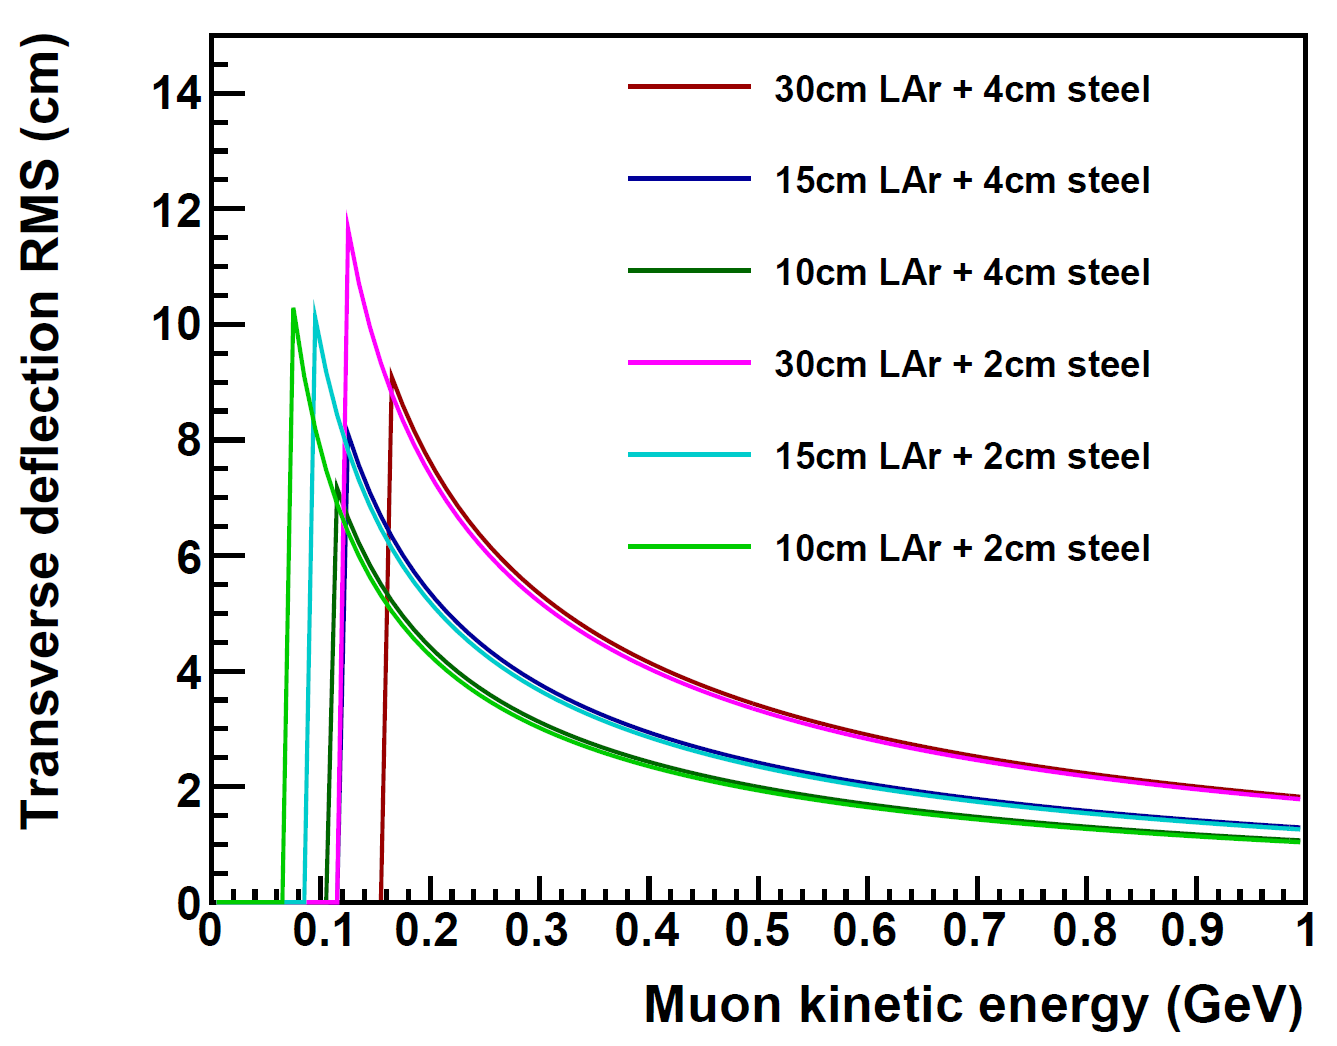
\includegraphics[width=0.65\textwidth]{graphics/mu_multiscat_rms.png}
\end{dunefigure}

\begin{dunefigure}[Fraction of total cross section with less than 10\% efficiency compared to ProtoDUNE]{fig:eff_numucc_10pct_protodune}
{The uniform cryostat walls in Figure 4 are compared to a scenario with 100 $\mbox{g}/\mbox{cm}^2$ total for thin regions, but where only 16\% of the downstream wall area is more than 10 cm away from any steel beam in a ProtoDUNE-like cryostat.}
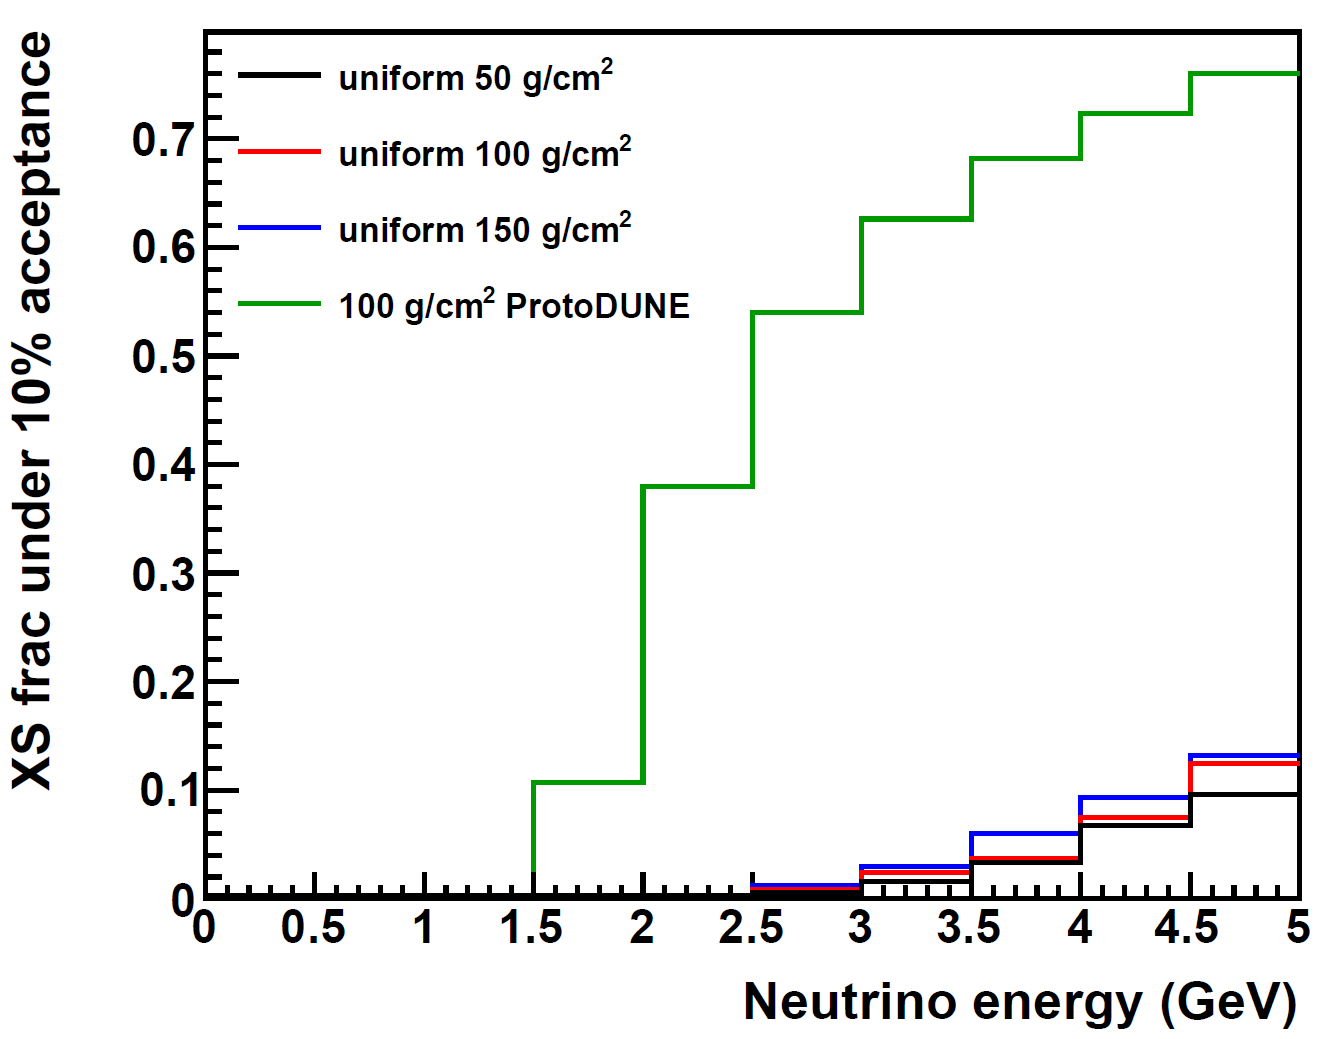
\includegraphics[width=0.65\textwidth]{graphics/numu__cc_efficiency_10pct_protodune.png}
\end{dunefigure}


\subsubsubsection{Cryostat Wall Unifomity}
In addition to being sufficiently thin to preserve high-acceptance regions for CC $\nu_\mu$ interactions, the energy loss in the cryostat wall must be modeled, so that it can be added back to the energy estimate for tracks that are matched to the spectrometer. This places a requirement on the uniformity of the cryostat wall; if the wall is non-uniform, then it will introduce a smearing on this piece of the correction that may worsen the muon energy resolution beyond the requirement. The lowest momentum muons that will be analyzed by matching tracks to the spectrometer are about 600 MeV. This number assumes the maximum allowed passive material, and includes the 150 cm traversed in liquid argon. That muon will lose about 200 MeV in the passive material, about 100 MeV of which is in the ND-LAr passive material including the cryostat wall. We use the 4\% momentum resolution requirement to define a maximum uncertainty on the energy loss in the passive material of 24 MeV for a 600 MeV muon. Half of that would come from the ND-LAr cryostat and other passive material, or 12 MeV. Compared to a 50 g/cm2 thickness, that is a uniformity requirement of 12\% across the downstream face of the detector.

\subsubsubsection{Adding Support Beams}
We can tolerate higher nonuniformity if it is confined to a relatively small fraction of the overall 7 X 3 m active area. For example, a 10 cm wide steel support running down the middle of the downstream face of the cryostat could be mitigated in analysis by simply excluding muons that pass through it with minimal loss of physics coverage. The areal density integrated along a straight-line trajectory connecting the two active detectors is then irrelevant because the muons will be rejected anyway. If the 60 g/cm2 requirement cannot be met with a uniform cryostat wall, it is preferable to add support beams over a small fraction of the wall area, while keeping the majority of the area below 60 g/cm2, see Figure \ref{fig:eff_numucc_10pct}.

In this scenario, muons that pass very near the dense support structures will be excluded from analysis. It is critical that we are able to correct the muon energy for losses event by event, which will not be possible for muons that pass very near the dense regions as small deviations in their position will lead to large changes in energy loss. Due to multiple scattering in the passive material itself, a buffer around the beams is required. Uninstrumented LAr on the cold side of the cryostat is especially important, because small angular deflections there are amplified by the long lever arm of the insulating foam. Figure \ref{fig:mu_multiscat_rms} shows the expected RMS of the transverse deflection at the face of the spectrometer due to muon multiple scattering in the LAr cryostat. It assumes some uninstrumetned LAr, followed by a 2 mm stainless steel inner membrane, 80 cm of polyurethane insulating foam, and a steel outer membrane, followed by a 10 cm air gap. Muon energy loss is accounted for, and the turn-off at low energy in each configuration is due to muons that range out in the cryostat.

A 10 cm buffer around any beams is sufficient to account for multiple scattering, except possibly at very low muon energy. For a cryostat wall with many steel beams like the SBND or ProtoDUNE designs, this results in a significant loss of events. To cut at least 10 cm away from all beams and stiffeners creates four ~20 X 20 cm2 squares in every 1 X 1 m2 of total area, resulting in a reduction factor of 16\%. Applying that to the acceptance, the fraction of the cross section phase space with very low acceptance below 10\% is much higher than for a uniform wall, as shown in Figure \ref{fig:eff_numucc_10pct_protodune}.

This loss in acceptance could be mitigated in two ways. First, effort should be made to increase the spacing between beams. A steel outer membrane of a few cm with larger beam spacing could create significantly larger square regions in between beams where events would be accepted. Second, these squares could be instrumented outside the outer membrane, to potentially tag muons that do not intersect beams. This may allow a reduction in the 10 cm buffer around the beams to account for multiple scattering if the non-beam-traversing events can be efficiently tagged. The feasibility of this should be further studied with simulation.

These vertical beams will create acceptance differences as a function of the horizontal position of the event, which corresponds to the off-axis position in the PRISM analysis. The flux changes as a function of off-axis position become significant at the 50cm level, so the width of any single support should be less than half of that, or 25 cm. The total width of the supports should not exceed 10\% of the area of the downstream face. The remaining 90\% of the area must meet the 12\% uniformity requirement. The position resolution will be degraded by the presence of passive argon between the active region and the cryostat wall, so it will not be possible to exclude muons that pass through the supports event by event if the gaps between the supports are too small. For that reason, there should be as few support beams as possible while meeting the other requirements stated above.

\subsubsubsection{Composite Window Construction}

\subsubsubsection{Progressive Prototyping Plan}

\subsubsection{Procurement}

\subsubsection{Infrastructure and Tooling}

\subsubsection{Auxiliary Pieces and Instillation}


%%%%%%%%%%%%%%% one subsec for each wbs element
\subsection{Membrane Cryostat Safety}
\label{sec:cryost-des-safety}

\begin{itemize}
\item FNAL membrane cryostat safety standards
\item LBNL cryostat analyses per FNAL standards
\item Cryostat pressure relief per FNAL standards
\end{itemize}


%%%%%%%%%%%%%%% one subsec for each wbs element
\subsection{Warm Structure}
\label{sec:cryost-des-warm}
The steel warm structure is constructed from wide flange I-beams that are welded into wall/floor structures and then bolted together; these provide mechanical support to both the cold membrane and insulation.  The 10mm steel skin is welded to the I-beams, as well as adjacent skins to form a vapor barrier.  This external steel structure provides the mechanical support required against the liquid argon hydrostatic load, argon-gas overpressure load, gravitational loads, and external constraints. The design intent is to provide a support surface flatness for the membrane cryostat within +/- 5mm.
The warm structure base interfaces to a steel beam platform, which itself interfaces to a linear rail-system for translating the entire structure along the length of the underground cavern.
The warm structure’s leak integrity is be verified prior to cold structure installation.  Qualification activities may include, but are not limited to, the following:
\begin{enumerate}
    \item Dye Penetrant Analysis
    \item Helium Leak Rate Measurement 
\end{enumerate}
Responsibility for qualification of the warm structure rests with LBNL and the DUNE-ND Project.

%\begin{itemize}
%\item Exterior steel skin \& steel beams
%\item Composite window
%\end{itemize}

%%%%%%%%%%%%%%% one subsec for each wbs element
\subsection{Cold Structure}
\label{sec:cryost-des-cold}
\subsubsection{Cold Structure}
The cold vessel design utilizes the stainless steel membrane technology. The thermal insulation requirements necessitate a nominal insulation thickness equal to 800mm (an insulation thickness of 600mm would be desirable if the RHI requirement (<10 W/m2) can be satisfied).  The cold membrane and insulating structure provides both a primary and secondary membrane for two levels of liquid containment.  Liquid argon containment at the boundary of the warm steel structure is not required.  A 10mm thick, leak-tight steel skin is present behind the insulation and acts as a vapor barrier from the ambient environment and as an enclosure for circulated nitrogen gas.

%\begin{itemize}
%\item Primary containment membrane \& insulation
%\item Secondary containment membrane \& insulation
%\end{itemize}

%%%%%%%%%%%%%%% one subsec for each wbs element
\subsection{Cryostat Lid (roof?)}
\label{sec:cryost-des-lid}
\subsubsection{Cryostat Lid}
The cryostat lid is segmented into three main sections: cryogenic services, LArTPC module support and services, and pressure relief end section.  The cryogenics section is installed first and provides liquid and gaseous argon services to the main cryostat volume.  The LArTPC sections provide mechanical support for the detector modules; as well as penetrations for detector signal and power routing, and high voltage delivery.  After the cryogenic section is installed, the LArTPC detector sections are sequentially installed to the main body of the cryostat.  A weld seam is laid down to seal the internal argon environment from atmosphere followed by brackets that bolts into place and complete the required load transfer for structural support.  The cryostat lid sections are comprised of a 10mm steel plate and beam structure, similar to the cryostat warm structure main body.  The top cap shall have a nominal insulation thickness of 800 mm and an internal stainless steel cold membrane on the bottom surface; however it is not envisioned that this surface is corrugated.

%\begin{itemize}
%\item Cryogenic Services Section
%\item LAr TPC Module Sections
%\item Final Lid Section - Cryo Pressure Relief
%\end{itemize}

%%%%%%%%%%%%%%% may not be needed?
\subsection{Infrastructure and Tooling}
\label{sec:cryost-des-infr}

%%%%%%%%%%%%%%% may be wbs elements?
\subsection{Auxiliary Pieces and Instrumentation}
\label{sec:cryost-des-aux}

%%%%%%%%%%%%%%%%%%%%%%%%%%%%%%%%
\section{Interfaces}
\label{sec:cryost-interface}

Table~\ref{tbl:cryost-interfaces} contains a summary and brief description of all the interfaces between the cryostat consortium and other consortia, working groups, and task forces, with references to the current version of the interface documents describing those interfaces.  
Drawings of the mechanical interfaces and diagrams of the electrical interfaces are 
included in the interface documents as appropriate.
It is expected that further refinements of the interface documents will take place prior to the final \dword{prr} for the detector. The interface documents specify the responsibility of different consortia or groups during all phases of the experiment including design and prototyping, integration,  installation, and  commissioning.


\begin{dunetable}
[Cryostat interface links]
{p{0.25\textwidth}p{0.5\textwidth}l}
{tbl:cryost-interfaces}
{cryostat interface links}
Interfacing System & Description & Linked Reference \\ \toprowrule
\dword{ndlar}      &  (desc)
& \citedocdb{?} \\ \colhline

\dshort{duneprism} (cryostat movement) &  (desc)
& \citedocdb{?} \\ \colhline

\dshort{lbnf}  cryogenics &  (desc)
& \citedocdb{?} \\ \colhline

\dshort{tms}  &  (desc)
& \citedocdb{?} \\ \colhline

Near Site I\&I &  (desc)
& \citedocdb{?} \\ \colhline

\dshort{daq}     &  (desc) 
 & \citedocdb{?} \\
\end{dunetable}



%%%%%%%%%%%%%%%%%%%%%%%%%%%%%%%%
\section{Risks and Mitigations}
\label{sec:cryost-risks}

Table~\ref{tab:table-cryost-risks} contains a list of all the
risks that \dword{dune} is currently holding in the cryostat risk register.  Each line includes the official \dword{dune} risk register identification number, a description of the risk, the proposed mitigation for the risk, and finally three columns rating the post-mitigation (P)robability that the risk described comes to pass, the degree of (C)ost risk for that line, and the degree of (S)chedule risk.  Risk levels are defined as (L)ow (<10\% probability of occurring, <5\% cost impact, <2 month schedule impact), (M)edium (10 to 25\% probability of occurring, 5\% to 20\% cost impact, 2 to 6 month schedule impact), or (H)igh (>25\% probability of occurring, >20\% cost impact, >6 month schedule impact).  Most of these risks are reduced to a ``Low'' level following mitigation (as shown in the table), although several of them currently hold a higher risk levels (pre-mitigation), due to the early stage of development of the cryostat system relative to other systems.  

In the following sections, we present a narrative description of each of the risks and the proposed mitigation.

\fixme{Anne needs to get risk table template put together}
%\input{generated/risks-longtable-ND-LAr.tex}

\begin{itemize}
\item Membrane cryogen leak
\item Ambient moisture leak
\end{itemize}

\begin{dunetable}
[Placeholder for risks table]
{cc}
{tab:table-cryost-risks}
{Placeholder for Risks Table - it will be generated from a spreadsheet}
Rows & Counts \\ \toprowrule
Row 1 & First \\ \colhline
Row 2 & Second \\ \colhline
Row 3 & Third \\ % no \colhline on final row
\end{dunetable}

%%%%%%%%%%%%%%%%%%%%%%%%%%%%%%%%
\section{Schedule}
\label{sec:cryost-org-sched}

Table \ref{tab:cryost-sched} lists key milestones in the design, validation, construction, and installation of the cryostat.  These milestones include external milestones indicating linkages to the main \dword{dune} schedule (highlighted in color in the table), as well as internal milestones such as design validation and technical reviews.

\fixme{Anne to get list of main DUNE sched items from Eric J before making the real table template}


\begin{itemize}
\item Warm structure
\item Cold structure
\item Composite window
\item Cryostat lid
\item Cryostat integration at Near Site
\end{itemize}

\begin{longtable}
{p{0.75\textwidth}p{0.25\textwidth}}
\caption{Cryostat consortium schedule}\\ \colhline
\rowcolor{dunetablecolor}Milestone & Date   \\ \toprowrule


\rowcolor{dunepeach}Beneficial occupancy of cavern 1 and \dword{cuc}& \cucbenocc      \\ \colhline
Initial batch (80 PD modules) assembled  & March 2023\\ \colhline

\rowcolor{dunepeach}Top of \dword{detmodule} \#1 cryostat accessible& \accesstopfirstcryo      \\ \colhline
Third batch (320 PD modules) arrive at US PD Reception Facility  & January 2024\\ 

\label{tab:cryost-sched}
\end{longtable}

%%%%%%%%%%%%%%%%%%%%%%%%%%%%%%%%
\section{Prototyping Plans}
\label{sec:cryost-proto}

Progressive prototypes for composite wall

%%%%%%%%%%%%%%%%%%%%%%%%%%%%%%%%
\section{Construction Plans}
\label{sec:cryost-construc}


\begin{itemize}
\item Warm structure installation
  \begin{itemize}
  \item Steel section assembly
  \item  Composite wall installation
  \end{itemize}
\item Cold structure installation
  \begin{itemize}
  \item Primary membrane \& insulation
  \item  Secondary membrane \& insulation
  \end{itemize}
\item Cryostat lid installation
\item Leak checking
\item Commissioning
\end{itemize}

\begin{comment} %% commenting all to the end
\fixme{The following sections are not in the new structure; I'm keeping them at the end here for now, in case you want to include one or more of them later.}
%%%%%%%%%%%%%%%%%%%%%%%%%%%%%%%%Not in Tim's new organization
\section{Safety Concerns}
\label{sec:cryost-safety}

%%%%%%%%%%%%%%%%%%%%%%%%%%%%%%%%Not in Tim's new organization
\section{Calibration}
\label{sec:cryost-calib}

%%%%%%%%%%%%%%%%%%%%%%%%%%%%%%%%Not in Tim's new organization
\section{Quality Assurance}
\label{sec:cryost-qa}


%%%%%%%%%%%%%%%%%%%%%%%%%%%%%%%%Not in Tim's new organization
\section{Transport and Handling}
\label{sec:cryost-transport}

%%%%%%%%%%%%%%%%%%%%%%%%%%%%%%%%Not in Tim's new organization
\section{Installation, Integration, and Commissioning}
\label{sec:cryost-iic}

%%%%%%%%%%%%%%%%%%%%%%%%%%%%%%%%Not in Tim's new organization
\section{Organization}
\label{sec:cryost-org}

%%%%%%%%%%%%%%%Not in Tim's new organization
\subsection{Participating Institutions}
\label{sec:fdsp-org-inst}
%\metainfo{\color{red}\bf  Content: Segreto/Warner}

The cryostat consortium benefits from the contributions of many institutions and facilities in \fixme{several countries? or the U.S. and ??}.  Table~\ref{tab:cryost-institutes}
lists the member institutions. 

\begin{longtable}
{ll}
\caption{Cryostat consortium institutions}\\ \colhline
\rowcolor{dunetablecolor} Member Institute  &  Country       \\  \toprowrule
univ 1 &  \\ \colhline
univ 2 &  \\ \colhline
univ 3 &  \\ 
\label{tab:cryost-institutes}
\end{longtable}

\end{comment}










